\section{Results}


\begin{figure}[h!]
    \centering
    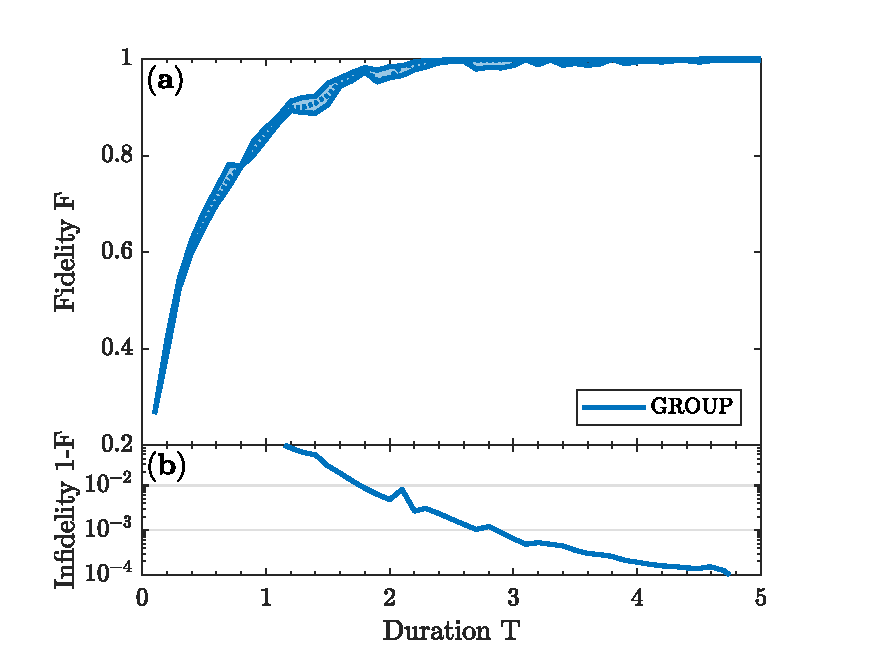
\includegraphics[width=0.45\textwidth]{Figures/FidelityDuration.pdf}
    \caption{\textit{Final fidelity obtained for optimal control at various durations. \textbf{(a)} the dotted line marks the median fidelity achieved, while the shaded area displays the $25\%$- and $75\%$-quartiles of the solutions. \textbf{(b)} the lowest infidelity achieved for each duration. }}
    \label{fig:FidelityDuration}
\end{figure}

\begin{figure}[h!]
    \centering
    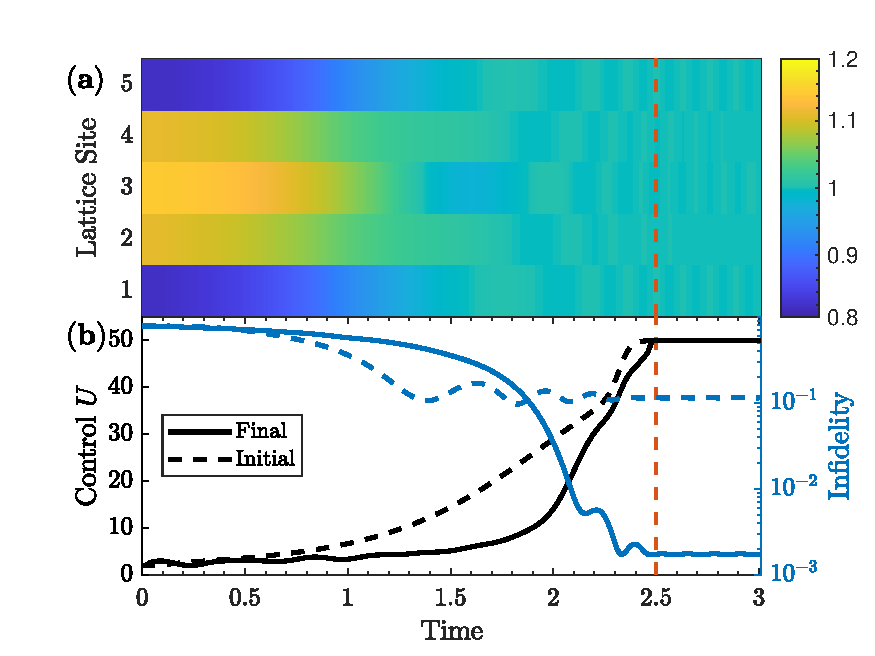
\includegraphics[width=0.45\textwidth]{Figures/OptRamp.pdf}
    \caption{\textit{Solution with highest fidelity achieved for duration $T = 2.5$. The dashed, red line marks the end of the duration, from which the system is further evolved using the final control value. \textbf{(a)} logarithmically scaled expectation value of the number operator, $\braket{\hat{n}_i}$, for each site, as the system is evolved according to the optimized ramp. \textbf{(b)} the initial and optimized ramp sequences along with the corresponding evolution of fidelities.}}
    \label{fig:OptRamp}
\end{figure}

\begin{figure}[h!]
    \centering
    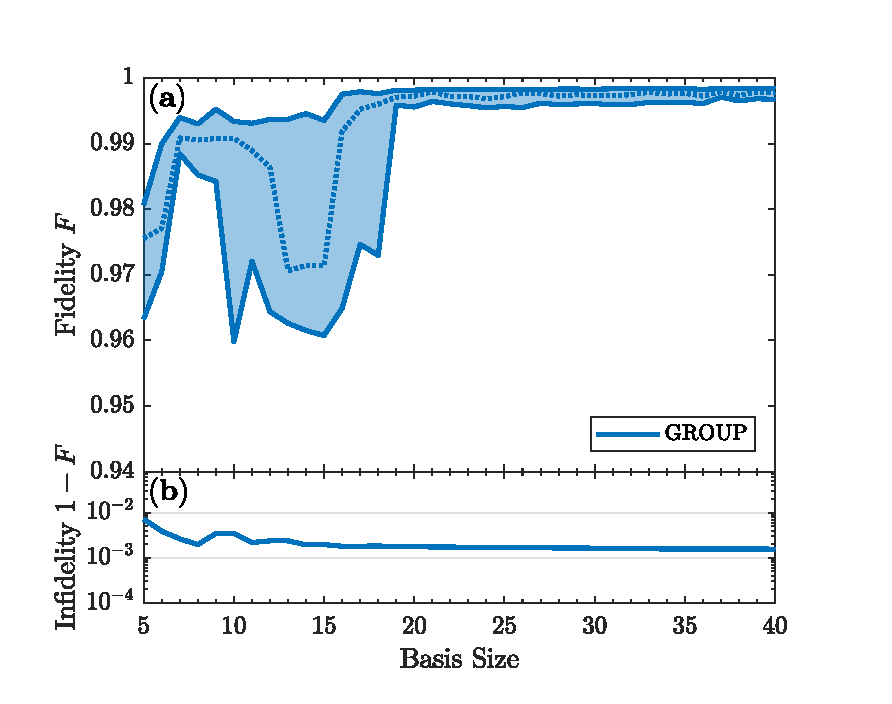
\includegraphics[width=0.45\textwidth]{Figures/FidelityBasisSize.pdf}
    \caption{\textit{Final fidelity obtained for optimal control at various optimization space dimensions for duration $T = 2.5$. \textbf{(a)} the dotted line marks the median fidelity achieved, while the shaded area displays the $25\%$- and $75\%$-quartiles of the solutions. \textbf{(b)} the lowest infidelities achieved for each basis size.}}
    \label{fig:FidelityBasisSize}
\end{figure}

\begin{figure}[h!]
    \centering
    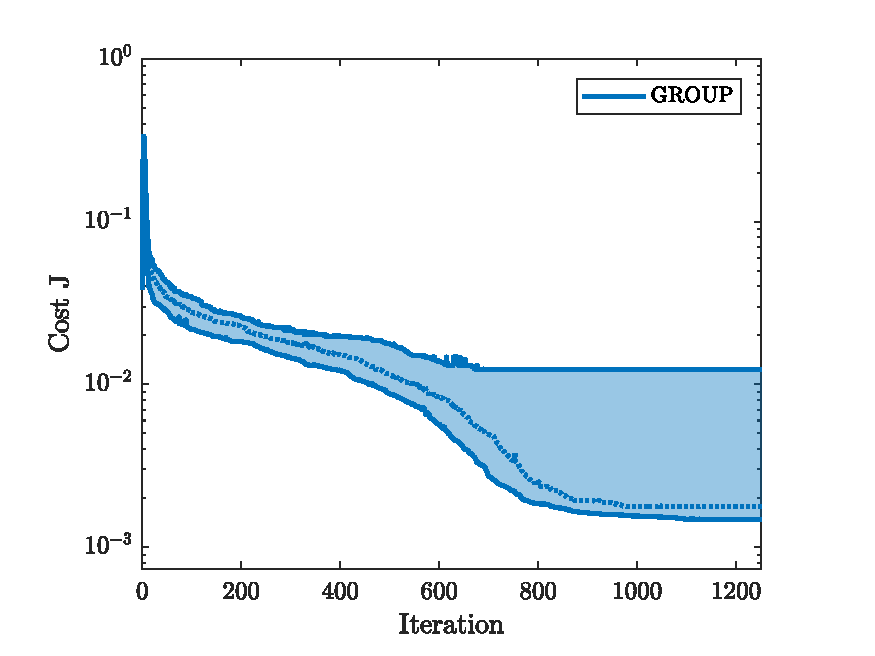
\includegraphics[width=0.45\textwidth]{Figures/CostProgress.pdf}
    \caption{\textit{The value of the cost function at a given number of time evolutions. The dotted line marks the median and the shaded area indicates the $25\%$- and $75\%$-quartiles found from X different random initial controls.}}
    \label{fig:FidelityBasisSize5}
\end{figure}